\documentclass[11pt, a4paper]{beamer}
\usepackage{amsmath}
\usepackage{amsfonts}
\usepackage{amssymb}
\usepackage{tikz}
\usepackage{multirow}

\usetheme{Frankfurt}
\usecolortheme{seagull}
\usepackage{xltxtra,fontspec}
\usepackage{polyglossia}
\setmainlanguage{german}
\defaultfontfeatures{Scale=MatchLowercase}

\usepackage[absolute,overlay]{textpos}

\setbeamertemplate{footline}
{
  \leavevmode%
  \hbox{%
  \begin{beamercolorbox}[wd=.4\paperwidth,ht=2.25ex,dp=1ex,center]{author in head/foot}%
    \usebeamerfont{author in head/foot}\insertshortauthor
  \end{beamercolorbox}%
  \begin{beamercolorbox}[wd=.6\paperwidth,ht=2.25ex,dp=1ex,center]{title in head/foot}%
    \usebeamerfont{title in head/foot}\insertshorttitle\hspace*{3em}
    \insertframenumber{} / \inserttotalframenumber\hspace*{1ex}
  \end{beamercolorbox}}%
  \vskip0pt%
}


\setbeamertemplate{navigation symbols}{}

\author{J. Nathanael Philipp, Felix Rauchfuß, Kai Trott}
\title{TIMA}
\date{25. Juli 2015}
\institute{Universität Leipzig}

\logo{
	
\includegraphics[scale=0.1]{./tima.png}
	\vspace{0.1cm}\hspace{0.2cm}
}
%\setbeamersize{text margin left=7mm, text margin right=7mm}

\begin{document}
\section{}
\begin{frame}
\titlepage
\end{frame}

\begin{frame}{Outline}
	\tableofcontents
\end{frame}

\section{What is TIMA?}
\begin{frame}{TIMA}
	\begin{itemize}
		\item TIMA is my association
		\item Database for associations
		\item Website \& Apps
	\end{itemize}
\end{frame}

\section{Website}
\subsection{Website}
\begin{frame}{Website}
	\begin{itemize}
		\item Main part
		\item Input for associations
		\item Usermanagement
		\item API
		\begin{itemize}
			\item OAuth2
			\item OAI-PMH
		\end{itemize}
	\end{itemize}
\end{frame}

\subsection{Data model}
\begin{frame}
	\begin{center}
		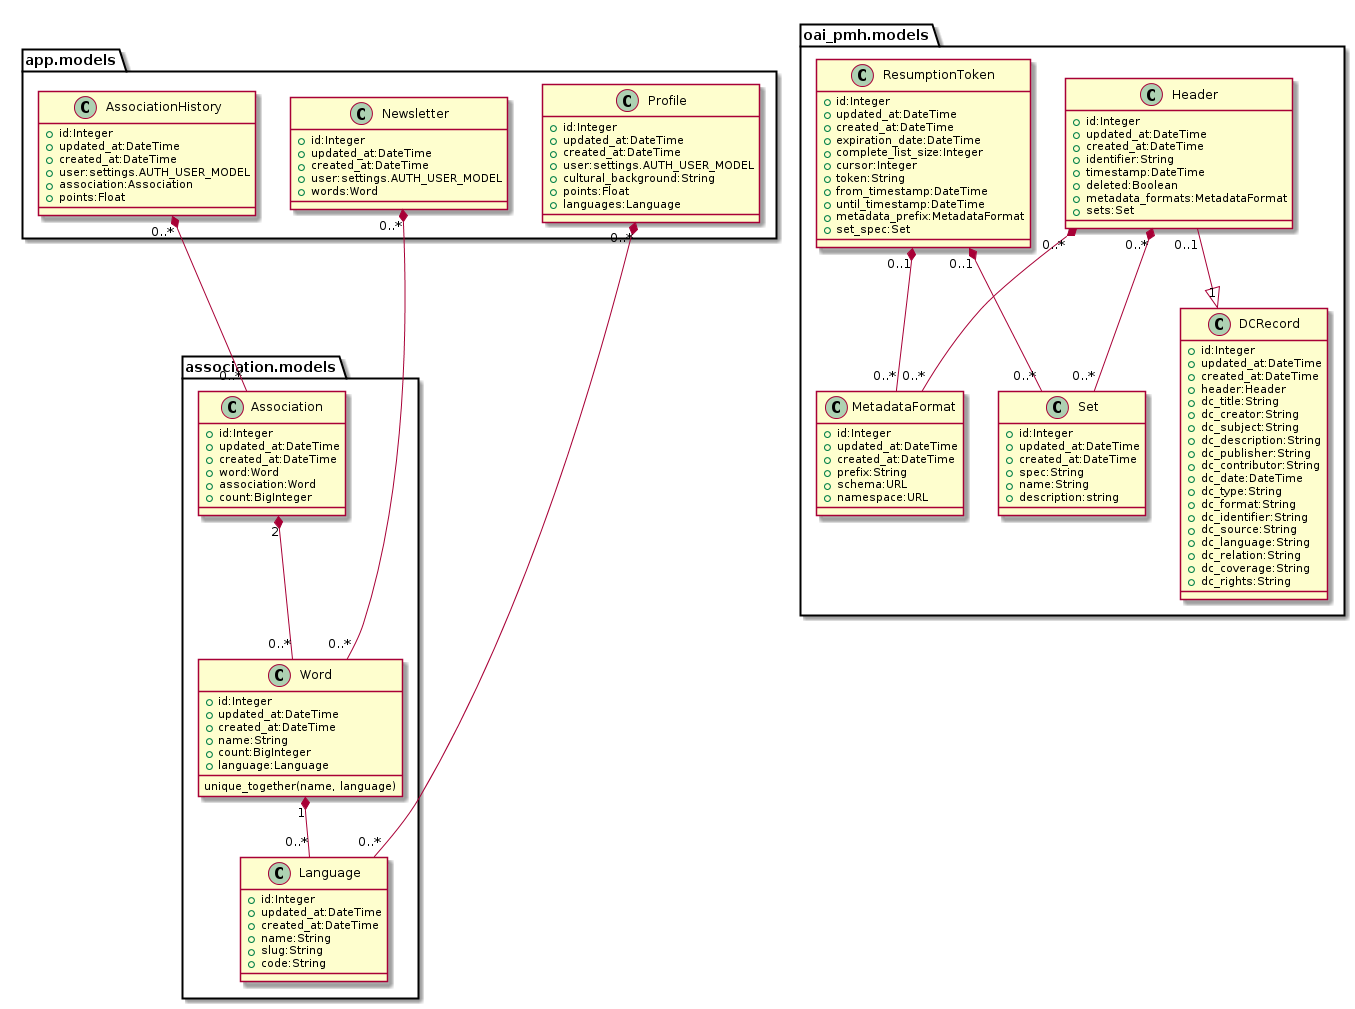
\includegraphics[width=\textwidth]{uml.png}
	\end{center}
\end{frame}

\end{document}